\chapter{Los compuestos organomagnesianos}\label{ch:b1:organomagnesium}

La mayoría de las moléculas orgánicas útiles tienen más átomos de carbono
que cualquier materia prima barata, y el problema central de la síntesis
es unir dos esqueletos carbonados mediante un nuevo enlace C--C. En un
compuesto de carbono, el carbono es casi siempre el participante pobre
en electrones de un enlace --- con el oxígeno, con un halógeno ---, y dos
carbonos pobres en electrones no reaccionan entre sí. A comienzos del
siglo XX, un reactivo preparado en un solo matraz a partir de un
halogenoalcano y magnesio dio la vuelta a esta situación: su carbono es
rico en electrones, un \omterm{def:b1:electronic-effects:nucleophile}{nucleófilo} que ataca el carbono de un grupo
carbonilo. Con él pueden construirse, a partir de piezas más pequeñas,
alcoholes de casi cualquier esqueleto. Este capítulo muestra cómo se
prepara el reactivo, por qué necesita un matraz perfectamente seco, a qué
se adiciona y cómo planificar con él.

\begin{recall}
La \omterm{def:b1:periodicity:electronegativity}{electronegatividad} (\cref{ch:b1:periodicity}); los ácidos y \omterm{def:b1:lewis-resonance-vsepr:lewis-acid}{bases de
Lewis} y el \omterm{def:b1:lewis-resonance-vsepr:lewis-acid}{enlace dativo} (\cref{ch:b1:lewis-resonance-vsepr}); los
\omterm{def:b1:electronic-effects:nucleophile}{nucleófilos}, los \omterm{def:b1:electronic-effects:nucleophile}{electrófilos}, las \omterm{def:b1:electronic-effects:curly-arrow}{flechas curvas} y la escala de
$\mathrm{p}K_a$ de las especies orgánicas (\cref{ch:b1:electronic-effects});
la clase de un alcohol (primario, secundario, terciario) es la de su
carbono.
\end{recall}

\section{Preparar un reactivo de Grignard}

\begin{definition}[Compuesto organometálico, reactivo de Grignard]\label{def:b1:organomagnesium:organometallic}
Un \emph{compuesto organometálico}\index{compuesto organometalico@compuesto organometálico} contiene al
menos un enlace carbono--metal. Un \emph{compuesto
organomagnesiano}\index{compuesto organomagnesiano} tiene un enlace C--Mg;
el \emph{reactivo de Grignard}\index{reactivo de Grignard} \ce{RMgX}
(X = Cl, Br, I), preparado a partir de un halogenoalcano o un
halogenoareno y magnesio en un éter, \ce{R-X + Mg -> R-MgX}, es el más
común.
\end{definition}

El magnesio se inserta en el enlace C--X. El éter no es un disolvente
inocente: el magnesio de \ce{RMgX} solo tiene cuatro \omterm{def:b1:quantum-numbers:configuration}{electrones de
valencia} a su alrededor, y dos moléculas de éter le ceden sus \omterm{def:b1:lewis-resonance-vsepr:lewis}{pares no
enlazantes}, completando su octeto y manteniendo el reactivo en
disolución.

\begin{omfigure}
\begin{tikzpicture}[font=\small]
  \node (mg) at (0,0) {Mg};
  \node (r) at (-1.5,0) {R};
  \node (x) at (1.5,0) {Br};
  \node (o1) at (0,1.45) {O};
  \node (o2) at (0,-1.45) {O};
  \draw[thick] (r) -- (mg) -- (x);
  \draw[thick, ->, omDef] (o1) -- (mg);
  \draw[thick, ->, omDef] (o2) -- (mg);
  \draw (o1) -- ++(-0.8,0.45) node[left] {\ce{CH3CH2}};
  \draw (o1) -- ++(0.8,0.45) node[right] {\ce{CH2CH3}};
  \draw (o2) -- ++(-0.8,-0.45) node[left] {\ce{CH3CH2}};
  \draw (o2) -- ++(0.8,-0.45) node[right] {\ce{CH2CH3}};
  \node[align=left, anchor=west] at (3.2,0) {dos moléculas de éter ceden\\cada una un par no\\enlazante (en azul):\\magnesio tetraédrico,\\octeto de electrones};
\end{tikzpicture}

{\small Un \omterm{def:b1:organomagnesium:organometallic}{reactivo de Grignard} en etoxietano (éter dietílico). Los
\omterm{def:b1:lewis-resonance-vsepr:lewis-acid}{enlaces dativos} oxígeno--magnesio explican por qué el reactivo solo se
forma en un éter o en una \omterm{def:b1:lewis-resonance-vsepr:lewis-acid}{base de Lewis} análoga.}
\end{omfigure}

\begin{method}[Preparar un reactivo de Grignard]\label{met:b1:organomagnesium:prepare}
\begin{enumerate}
  \item Se seca en la estufa todo el material de vidrio; se coloca en el
        refrigerante un tubo desecante de cloruro de calcio; se usa un
        éter anhidro.
  \item Se ponen las virutas de magnesio y un poco de éter en un matraz de
        tres bocas provisto de refrigerante, embudo de adición y
        agitador.
  \item Se añade una pequeña porción del haluro; cuando empieza la
        reacción (turbidez, ebullición suave del éter), se añade el resto
        gota a gota a un ritmo que mantenga un reflujo suave.
  \item La disolución se usa de inmediato, en el mismo montaje seco.
\end{enumerate}
\end{method}

\begin{omfigure}
\begin{tikzpicture}[font=\small]
  \pic at (0,-0.05) {stirrer};
  \pic (f) at (0,0.05) {threeneck={0.35}{omDef!14}};
  \pic at (f-c) {condenser};
  \pic at ($(f-c)+(0,3.2)$) {guardtube};
  \pic[rotate=25] at (f-l) {dropfunnel={0.5}{orange!20}};
  \fill[black!45, rotate around={-25:(f-r)}] ($(f-r)+(-0.17,0)$) rectangle ++(0.34,0.3);
  \draw[->] (2.4,0.9) node[right] {virutas de Mg en éter seco} -- (0.6,0.6);
  \draw[->] (-3.0,3.9) node[left, align=right] {haluro en éter,\\añadido gota a gota} -- (-1.8,3.4);
  \draw[->] (1.8,5.3) node[right] {refrigerante (agua)} -- (0.45,4.8);
  \draw[->] (1.8,6.6) node[right] {tubo desecante de cloruro de calcio} -- (0.3,6.4);
  \draw[->] (2.4,-0.2) node[right] {agitador magnético} -- (1.3,-0.2);
\end{tikzpicture}

{\small Montaje para una reacción de Grignard: se seca todo lo que puede
alcanzar el aire. El tubo desecante detiene el vapor de agua del aire; el
refrigerante devuelve al matraz el éter que hierve.}
\end{omfigure}

\begin{inthelab}[Una reacción que tiene que arrancar]
A veces una preparación de Grignard se niega a arrancar: el magnesio está
cubierto por una película de óxido. Aplastar una viruta con una varilla
de vidrio, añadir un \omterm{def:b1:crystals-metals:crystal}{cristal} de yodo o calentar localmente el matraz deja
al descubierto metal limpio. Una vez iniciada, la reacción es exotérmica y
el éter hierve solo; entonces se ralentiza la adición para que no se
desborde. El etoxietano hierve a \qty{35}{\celsius} y su vapor es muy
inflamable: ninguna llama en todo el laboratorio, y un baño de hielo a
mano.
% ledger: bp:diethylether
\end{inthelab}

\section{Una base fuerte y un nucleófilo}

\begin{definition}[Inversión de polaridad]\label{def:b1:organomagnesium:umpolung}
La \omterm{def:b1:periodicity:electronegativity}{electronegatividad} del magnesio (1.31) es mucho menor que la del
carbono (2.55): en \ce{R-MgX}, el enlace C--Mg está polarizado con el
extremo negativo en el carbono, que se comporta como un \omterm{def:b1:electronic-effects:intermediates}{carbanión}. En el
haluro \ce{R-X}, el mismo carbono era positivo (X: 2.96 para el Br).
Convertir un carbono \omterm{def:b1:electronic-effects:nucleophile}{electrófilo} en uno \omterm{def:b1:electronic-effects:nucleophile}{nucleófilo} es una \emph{inversión
de polaridad}\index{inversion de polaridad@inversión de polaridad}.
% ledger: en:Mg, en:C, en:Br
\end{definition}

\begin{proposition}[Los hidrógenos ácidos destruyen los reactivos de Grignard]\label{prop:b1:organomagnesium:base}
Un \omterm{def:b1:organomagnesium:organometallic}{reactivo de Grignard} reacciona \omterm{def:b1:extent-q-and-k:quantitative}{cuantitativamente} con el agua, los
alcoholes, los ácidos carboxílicos, las aminas con enlaces N--H y los
alquinos terminales, y da el alcano
\ce{R-H}: \ce{RMgX + H2O -> R-H + Mg(OH)X}.
\end{proposition}

\begin{proof}
El carbono de tipo \omterm{def:b1:electronic-effects:intermediates}{carbanión} es la base del par \ce{R-H}/\ce{R^-}, y los
alcanos son con mucho los ácidos más débiles de la química orgánica:
no puede medirse en el agua que abandonen un protón, pues allí el
hidróxido es la base más fuerte que puede existir
(\cref{ch:b1:predominant-reaction}, \omterm{def:b1:predominant-reaction:levelling}{efecto nivelador}). Cualquier ácido de
la lista es mucho más fuerte, y la transferencia de protón a \ce{R^-}
tiene una constante enorme: es completa y rápida.
\end{proof}

Esta es la razón del montaje seco: una gota de agua destruye una cantidad
igual de reactivo. Convertido en ventaja, \ce{CH3CH2MgBr + D2O} sitúa un
átomo de deuterio exactamente donde estaba el bromo.

\section{Adiciones a compuestos carbonílicos y al dióxido de carbono}

El carbono de un grupo C=O es \omterm{def:b1:electronic-effects:nucleophile}{electrófilo} (\cref{ch:b1:electronic-effects}).
El \omterm{def:b1:organomagnesium:organometallic}{reactivo de Grignard} le adiciona su grupo R, y el par $\pi$ del C=O
pasa al oxígeno; un tratamiento ácido protona después el alcóxido.

\begin{omfigure}
\setchemfig{atom sep=2.1em}
\schemestart
\chemfig{@{r}R-[@{rm}]MgBr}
\+
\chemfig{@{cc}C(-[:150]R')(-[:210]R'')=[@{co}]@{o}O}
\arrow{->}
\chemfig{C(-[:150]R')(-[:210]R'')(-[2]R)-O^{-}}
\chemfig{\phantom{.}}\chemfig{^{+}MgBr}
\arrow{->[\ce{H3O+}]}
\chemfig{C(-[:150]R')(-[:210]R'')(-[2]R)-OH}
\schemestop
\chemmove{\draw[->, thick, shorten <=2pt, shorten >=2pt](rm) .. controls +(70:9mm) and +(180:7mm) .. (cc);
          \draw[->, thick, shorten <=2pt, shorten >=2pt](co) .. controls +(90:6mm) and +(90:6mm) .. (o);}
\par\vspace{6pt}

{\small Adición de un \omterm{def:b1:organomagnesium:organometallic}{reactivo de Grignard} a una cetona (o a un aldehído,
$\mathrm{R''} = \mathrm{H}$): el par C--Mg forma el nuevo enlace C--C
mientras el par $\pi$ del C=O pasa al oxígeno; el alcóxido de magnesio se
protona con ácido diluido en una etapa aparte.}
\end{omfigure}

\begin{proposition}[Alcoholes a partir de compuestos carbonílicos]\label{prop:b1:organomagnesium:carbonyl-addition}
Tras el tratamiento ácido, un \omterm{def:b1:organomagnesium:organometallic}{reactivo de Grignard} \ce{RMgX} da: con el
metanal, un alcohol primario \ce{RCH2OH}; con otro aldehído
$\mathrm{R'CHO}$, un alcohol secundario $\mathrm{RR'CHOH}$; con una
cetona $\mathrm{R'COR''}$, un alcohol terciario $\mathrm{RR'R''COH}$. El
nuevo enlace C--C une R al antiguo carbono carbonílico.
\end{proposition}

\begin{proof}
El carbono carbonílico conserva sus dos sustituyentes y gana R y un OH
(procedente del oxígeno del alcóxido): el metanal aporta dos H; un
aldehído, un H y un grupo carbonado; una cetona, dos grupos carbonados.
La clase del alcohol es el número de grupos carbonados de ese carbono:
uno, dos o tres.
\end{proof}

\begin{proposition}[Ácidos carboxílicos a partir del dióxido de carbono]\label{prop:b1:organomagnesium:co2}
Un \omterm{def:b1:organomagnesium:organometallic}{reactivo de Grignard} vertido sobre dióxido de carbono sólido da, tras
acidificar, el ácido carboxílico \ce{RCOOH}, con un carbono más:
\ce{RMgX + CO2 -> RCOOMgX} y, después,
\ce{RCOOMgX + H3O+ -> RCOOH + Mg^2+ + X- + H2O}.
\end{proposition}

\begin{proof}
\ce{CO2} es un compuesto carbonílico cuyo carbono es atacado como el de
una cetona; el carboxilato formado es demasiado poco reactivo para
adicionar un segundo grupo R en estas condiciones (un carbonilo con carga
negativa es un mal \omterm{def:b1:electronic-effects:nucleophile}{electrófilo}). El ácido lo protona.
\end{proof}

\section{Construir esqueletos carbonados}

\begin{method}[Planificar un alcohol]\label{met:b1:organomagnesium:plan-alcohol}
\begin{enumerate}
  \item Se localiza el carbono que lleva el OH en el alcohol buscado.
  \item Se elige uno de sus grupos carbonados como R (procederá del
        \omterm{def:b1:organomagnesium:organometallic}{reactivo de Grignard}, preparado a partir de \ce{R-Br}); el resto
        de la molécula, con ese carbono como C=O, es el participante
        carbonílico.
  \item Se enumeran las elecciones posibles (una por grupo carbonado) y se
        prefiere la que usa reactivos sencillos y disponibles.
  \item Se comprueba que ninguno de los dos participantes lleva un
        hidrógeno ácido o un segundo carbonilo que reaccionaría también.
\end{enumerate}
\end{method}

\begin{example}[El 2-fenilbutan-2-ol]\label{ex:b1:organomagnesium:plan}
El carbono que lleva el OH tiene un grupo fenilo, un metilo y un etilo.
Tres elecciones: bromuro de fenilmagnesio con butan-2-ona; bromuro de
metilmagnesio con 1-fenilpropan-1-ona; bromuro de etilmagnesio con
1-feniletan-1-ona (acetofenona). Las tres funcionan; la última usa dos de
los reactivos más corrientes.
\end{example}

\begin{history}[Victor Grignard]
\begin{minipage}[t]{0.2\linewidth}\vspace{0pt}
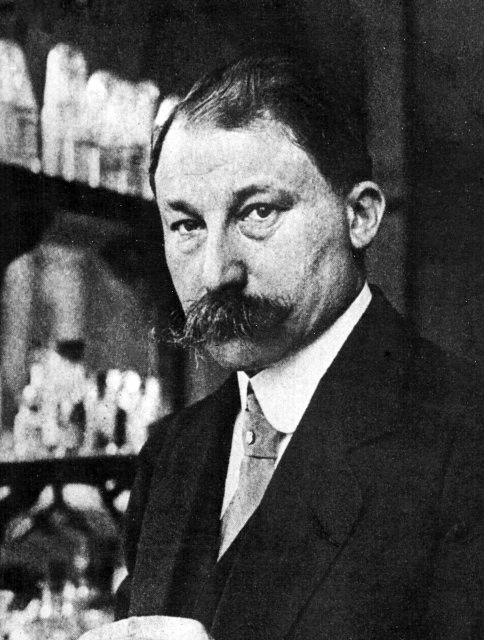
\includegraphics[width=\linewidth]{images/book2/grignard.jpg}
\end{minipage}\hfill
\begin{minipage}[t]{0.76\linewidth}\vspace{0pt}
El reactivo lleva el nombre de Victor Grignard, que, siendo estudiante
de doctorado a comienzos del siglo XX, descubrió que el magnesio se
disuelve en una disolución etérea de un halogenoalcano y que la
disolución se adiciona a los compuestos carbonílicos. Su sencillez ---
un metal, un disolvente, un matraz --- hizo de ella la reacción de
formación de enlaces carbono--carbono más usada del siglo, y le valió a su
descubridor un Premio Nobel de Química.
(Fotografía, dominio público, Wikimedia Commons.)
\end{minipage}
\end{history}

\section{Ejercicios}

\begin{exercise}[$\star$]\label{exo:b1:organomagnesium:1}
Escríbase la preparación del bromuro de etilmagnesio y del bromuro de
fenilmagnesio. Dese la polarización del enlace C--Br y la del enlace
C--Mg, con las \omterm{def:b1:periodicity:electronegativity}{electronegatividades}.
\end{exercise}

\begin{exercise}[$\star$]\label{exo:b1:organomagnesium:2}
¿Qué da el yoduro de metilmagnesio con: el agua; el etanol; el ácido
etanoico; el óxido de deuterio \ce{D2O}? Escríbanse las ecuaciones.
\end{exercise}

\begin{exercise}[$\star$]\label{exo:b1:organomagnesium:3}
Dese el producto (tras el tratamiento ácido) del bromuro de etilmagnesio
con el metanal, el etanal, la propanona, el benzaldehído y el dióxido de
carbono. Dese la clase de cada alcohol.
\end{exercise}

\begin{exercise}[$\star$]\label{exo:b1:organomagnesium:4}
¿Por qué no debe usarse el 4-bromobutan-1-ol para preparar un \omterm{def:b1:organomagnesium:organometallic}{reactivo de
Grignard}?
\end{exercise}

\begin{exercise}[$\star\star$]\label{exo:b1:organomagnesium:5}
Escríbanse con \omterm{def:b1:electronic-effects:curly-arrow}{flechas curvas} el mecanismo de la adición del bromuro de
metilmagnesio al etanal y el del tratamiento. ¿Es \omterm{def:b1:stereochemistry-in-depth:stereocentre}{quiral} el producto? ¿Se
obtiene como un solo enantiómero? ¿Por qué?
\end{exercise}

\begin{exercise}[$\star\star$]\label{exo:b1:organomagnesium:6}
Propónganse dos maneras de preparar el 3-metilpentan-3-ol a partir de un
\omterm{def:b1:organomagnesium:organometallic}{reactivo de Grignard} y una cetona.
\end{exercise}

\begin{exercise}[$\star\star$]\label{exo:b1:organomagnesium:7}
¿Cómo se prepararía el ácido 2-metilpropanoico a partir del
2-bromopropano? Calcúlese la masa de ácido que se obtiene a partir de
\qty{12.3}{g} de bromuro con un \omterm{def:b1:extent-q-and-k:fractional-extent}{rendimiento} del \qty{70}{\percent}
($M$: \ce{C3H7Br} \qty{123.0}{g/mol}, \ce{C4H8O2} \qty{88.0}{g/mol}).
\end{exercise}

\begin{exercise}[$\star\star$]\label{exo:b1:organomagnesium:8}
Un estudiante descuidado prepara bromuro de fenilmagnesio a partir de
\qty{0.0500}{mol} de bromobenceno en un éter que contiene \qty{0.18}{g} de
agua. ¿Qué fracción del reactivo se destruye? ¿Qué producto se forma?
\end{exercise}

\begin{exercise}[$\star\star$]\label{exo:b1:organomagnesium:9}
El bifenilo, \ce{C6H5-C6H5}, es un subproducto de la preparación del
bromuro de fenilmagnesio. Propóngase cómo se forma y por qué la adición
lenta del bromobenceno a un exceso de magnesio lo limita.
\end{exercise}

\begin{exercise}[$\star\star\star$]\label{exo:b1:organomagnesium:10}
Planifíquense dos síntesis del 1-feniletan-1-ol a partir de un \omterm{def:b1:organomagnesium:organometallic}{reactivo
de Grignard}, y una síntesis del 2-fenilpropan-2-ol. Para cada una,
nómbrese el haluro que da el reactivo.
\end{exercise}

\begin{exercise}[$\star\star\star$]\label{exo:b1:organomagnesium:11}
Explíquese por qué el \omterm{def:b1:organomagnesium:organometallic}{reactivo de Grignard} y el compuesto carbonílico
deben mezclarse en el orden elegido en el problema de abajo, y por qué el
tratamiento se hace con ácido diluido frío y no solo con agua.
\end{exercise}

\begin{exercise}[$\star\star\star$]\label{exo:b1:organomagnesium:12}
Se valora un \omterm{def:b1:organomagnesium:organometallic}{reactivo de Grignard} preparado a partir de \qty{0.100}{mol}
de un bromuro: se vierte una alícuota en un exceso de agua y la sal básica
de magnesio formada se valora con ácido clorhídrico; referidos a toda la
disolución, se necesitan \qty{0.088}{mol} de ácido. Explíquese el
principio y dese el \omterm{def:b1:extent-q-and-k:fractional-extent}{rendimiento} de la preparación.
\end{exercise}

\section{Problema: el trifenilmetanol}

\begin{problem}[{Problema de fin de semana --- la preparación del bromuro
de fenilmagnesio, su adición a la benzofenona, el tratamiento y el
rendimiento en trifenilmetanol}]
\label{pb:b1:organomagnesium:1}
En un matraz de tres bocas seco, \qty{0.535}{g} de magnesio y
\qty{3.14}{g} de bromobenceno en etoxietano anhidro dan bromuro de
fenilmagnesio. Después se añade gota a gota una disolución de
\qty{3.28}{g} de benzofenona, \ce{(C6H5)2CO}, en el mismo éter. Tras el
tratamiento con ácido sulfúrico diluido frío, la extracción y la
recristalización, se obtienen \qty{3.75}{g} de trifenilmetanol puro,
\ce{(C6H5)3COH}, y se separan \qty{0.15}{g} de bifenilo. Masas molares
(\unit{g/mol}): Mg 24.3, \ce{C6H5Br} 156.9, \ce{C13H10O} 182.0,
\ce{C19H16O} 260.0,
\ce{C12H10} 154.0, \ce{C7H6O2} 122.0.

\medskip
\noindent\textbf{Parte I --- El bromuro de fenilmagnesio.}
\begin{enumerate}
  \item Escríbase la ecuación de la preparación.
  \item Calcúlense las cantidades de magnesio y de bromobenceno. ¿Cuál
        está en exceso?
  \item ¿Por qué debe estar seco el montaje? Escríbase la reacción con el
        agua.
  \item ¿Cuál es la función del tubo desecante?
  \item ¿Por qué es esencial el éter, más allá de disolver los reactivos?
  \item El bifenilo procede de la reacción del reactivo con el
        bromobenceno. Escríbase y calcúlese la cantidad de bromobenceno
        perdida en ella.
\end{enumerate}

\medskip
\noindent\textbf{Parte II --- La adición.}
\begin{enumerate}[resume]
  \item Calcúlese la cantidad de benzofenona.
  \item Escríbase el mecanismo de la adición con \omterm{def:b1:electronic-effects:curly-arrow}{flechas curvas}.
  \item ¿Qué reactivo limita la formación de trifenilmetanol? Téngase en
        cuenta la parte I.
  \item ¿Es \omterm{def:b1:stereochemistry-in-depth:stereocentre}{quiral} el trifenilmetanol? Justifíquese.
  \item ¿Por qué se añade la benzofenona al reactivo y no al revés?
  \item ¿Qué haría una traza de agua en la disolución de benzofenona?
\end{enumerate}

\medskip
\noindent\textbf{Parte III --- El tratamiento.}
\begin{enumerate}[resume]
  \item Escríbase la protonación del alcóxido.
  \item ¿Por qué usar ácido diluido frío y no solo agua?
  \item ¿Dónde están el trifenilmetanol y las sales de magnesio tras la
        extracción con éter?
  \item ¿Cómo se separa el bifenilo del trifenilmetanol? (El bifenilo es
        mucho más soluble en éter de petróleo frío.)
  \item ¿Qué ensayo confirma la pureza de los \omterm{def:b1:crystals-metals:crystal}{cristales}?
  \item El trifenilmetanol resiste el ácido diluido frío, pero se disuelve
        en ácido sulfúrico concentrado dando un \omterm{def:b1:electronic-effects:intermediates}{carbocatión} de color
        amarillo intenso. Escríbase su formación y explíquese su
        estabilidad (compárese con el
        \cref{ch:b1:electronic-effects}).
\end{enumerate}

\medskip
\noindent\textbf{Parte IV --- El \omterm{def:b1:extent-q-and-k:fractional-extent}{rendimiento}, y otro producto.}
\begin{enumerate}[resume]
  \item Calcúlese la cantidad de trifenilmetanol obtenida.
  \item Calcúlese el \omterm{def:b1:extent-q-and-k:fractional-extent}{rendimiento} respecto del \omterm{def:b1:extent-q-and-k:max-extent}{reactivo limitante}.
  \item Propónganse dos causas de pérdidas.
  \item Si el reactivo de la parte I (corregido por el bifenilo) se hubiera
        vertido en cambio sobre dióxido de carbono sólido, ¿qué producto
        se formaría?
  \item Calcúlese la masa teórica de ese producto.
  \item Escríbase la ecuación de esa carboxilación.
  \item Dese el \omterm{def:b1:extent-q-and-k:fractional-extent}{rendimiento} en trifenilmetanol, en tanto por ciento.
\end{enumerate}
\end{problem}
